\documentclass[11pt]{article}
\usepackage[letterpaper,margin=1in]{geometry}
\usepackage[T1]{fontenc}
\usepackage{mathptmx}
\usepackage{graphicx}
\usepackage{booktabs}
\usepackage{tabularx}
\usepackage{amsmath}
\usepackage[hidelinks]{hyperref}
\usepackage[font=small,labelfont=bf]{caption}
\usepackage{enumitem}
\usepackage{titlesec}
\setlist{nosep,leftmargin=1.4em,topsep=2pt}
\titlespacing*{\section}{0pt}{9pt}{3pt}
\titleformat{\section}{\large\bfseries}{\thesection.}{0.5em}{}
\setlength{\parskip}{3pt}
\setlength{\parindent}{0pt}
\setlength{\textfloatsep}{8pt}
\setlength{\floatsep}{6pt}
\setlength{\intextsep}{6pt}
\pagestyle{plain}

\begin{document}

\begin{center}
{\LARGE\bfseries CIFAR-10 ResNet Under 5M Parameters: Project Report}\\[6pt]
{\large Team Transformers: Rishi Ajith and Kalp Patel}\\[2pt]
NYU Tandon School of Engineering, Deep Learning (Fall 2026), Project 1\\[2pt]
Code: \url{https://github.com/Kalp342/cifar10-resnet-5m}
\end{center}

\section*{Summary}
Our best model is a 4,918,602-parameter ResNet, trained from scratch, that scored \textbf{0.906 on the public leaderboard and 0.875 on the private leaderboard}. It is a student network distilled from four larger teachers we trained ourselves, refined by a model soup, and finally fine-tuned to reproduce the teacher ensemble's predictions on the unlabelled test images. Our two final submissions were this model and a second model soup (0.905 public, 0.867 private). Three lessons shaped the project:
\begin{enumerate}
\item \textbf{Distillation was the idea that mattered.} The 5M limit covers only the submitted model, so larger teachers were free capacity. Imitating them lifted the public score from 0.898 to 0.904, our largest single gain.
\item \textbf{The test set is shifted, and the teachers set the ceiling.} Our models reached 97.6--97.8\% on held-out CIFAR-10 images but only 87--91\% on the hidden ones. A distilled student lands just below its teachers on the shifted images, so the teachers decide how far a 5M student can go.
\item \textbf{The public leaderboard could not rank small ideas.} SAM, model soups and a high-resolution student each moved the public score by a few of its 1,000 images, inside its $\pm$1.9-point noise. Our last step gained 1 image publicly but 10 privately.
\end{enumerate}

\section{The task, and what made it hard}
The goal was the highest accuracy on 2,000 hidden CIFAR-10-style test images, using a ResNet trained from scratch with at most 5 million trainable parameters. No pretrained weights or outside data were allowed; any augmentation, optimizer, regularizer or distillation was. Half of the hidden images scored the public leaderboard and half the private one.

\textbf{The hidden images are harder than CIFAR-10 itself.} Our models scored 97.6--97.8\% on 5,000 training images we held out, but about 90\% on the public half and 86--88\% on the private half (Figure~\ref{fig:gap}). The test images are brighter and higher-contrast, and 3.3\% are near-grayscale versus 1.1\% in training; two of our models disagreed on 2.2\% of held-out images but on 7.5\% of test images. Recht et al.\ (2018) saw the same drop on a freshly collected CIFAR-10 test set: every model lost 4--10 points. Miller et al.\ (2021) showed that accuracy on such shifted sets rises in step with ordinary accuracy, so our working assumption was that the main way up was a more accurate model overall.

\textbf{The leaderboard is noisy.} With 1,000 images per half, one image is worth 0.1 points, and the 95\% confidence interval around a 90\% score is about $\pm$1.9 points. Our later submissions differed by only 1--10 images, so we treated small leaderboard changes as noise rather than evidence.

\begin{figure}[h]
\centering
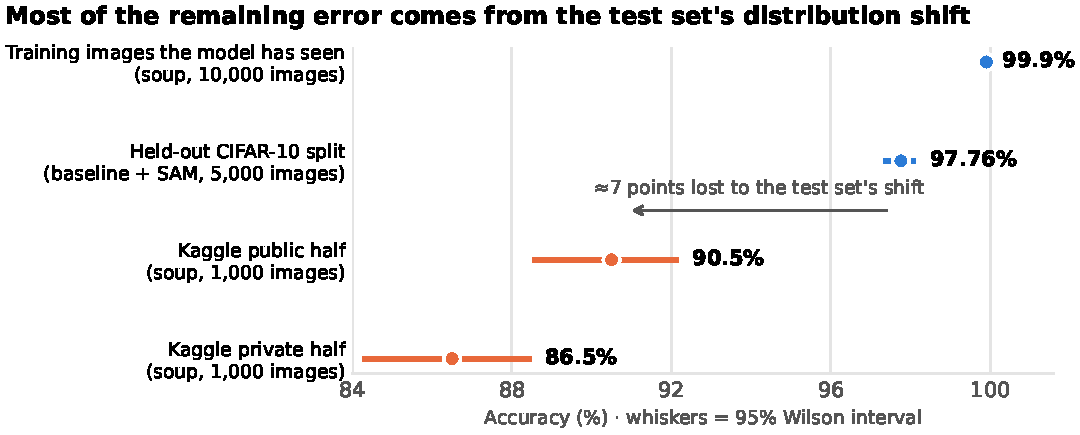
\includegraphics[width=0.88\linewidth]{fig1_accuracy_gap.pdf}
\caption{Accuracy on images the model trained on, on held-out CIFAR-10 images, and on both halves of the hidden test set. Whiskers are 95\% Wilson intervals; each leaderboard half has only 1,000 images, hence the wide intervals.}
\label{fig:gap}
\end{figure}

\section{Approach at a glance}
We kept one network design, a 3-stage ResNet under 5M parameters, and improved it over seven rounds, changing one idea at a time (Table~\ref{tab:rounds}). We tried the idea with the largest expected gain first, distillation, and cheaper refinements after it. In parallel, one of us built a separate pipeline (Wide ResNets distilled from our own, weaker teachers) whose best model scored 0.890; its main finding motivated round 6. Laptop GPUs throttled at 86--87\,\textdegree C and needed 45--108\,s per epoch; on A100 GPUs (NYU HPC and Colab) a distillation epoch took 8--20\,s, which made 500-epoch runs practical.

\begin{table}[h]
\centering\small
\caption{The rounds. Public and private scores use 1,000 images each; held-out accuracy uses 5,000 training images kept out of training.}
\label{tab:rounds}
\begin{tabularx}{\linewidth}{@{}clXl@{}}
\toprule
Round & Idea & What changed & Outcome \\
\midrule
0 & Baseline & 4.62M ResNet (3-4-3 blocks), 200 epochs, strong augmentation & 97.64\% held-out \\
1 & Distillation & Student copies the soft predictions of four larger teachers & 0.904 public \\
2 & Bigger teachers & Two 18.5M teachers; deeper 3-5-3 student (4.92M); 500 epochs & 0.904, closer to teachers \\
3 & SAM & Optimizer that seeks flat minima, same recipe & +0.12 held-out; 0.903 \\
4 & Model soup & Four fine-tuned copies of a student, weights averaged & 0.905 \\
5 & High-res student & Same 4.92M parameters, 3.1$\times$ compute per image & 0.903, most different \\
6 & Ensemble compression & Fine-tune the soup to match the teacher ensemble on the unlabelled test images & \textbf{0.906 / 0.875} \\
\bottomrule
\end{tabularx}
\end{table}

\section{Base network and training recipe}
The student is a 3-stage ResNet (He et al., 2016) built from basic residual blocks, $y = \mathrm{ReLU}(F(x) + S(x))$, where $F$ is conv3$\times$3 $\to$ BN $\to$ ReLU $\to$ conv3$\times$3 $\to$ BN, and $S$ is the identity or, where stride or width changes, a 1$\times$1 convolution plus BN. A stem (conv3$\times$3, BN, ReLU) feeds stages at 32$\times$32, 16$\times$16 and 8$\times$8 resolution, then global average pooling and a linear layer. With widths 64/128/256 and 3-5-3 blocks it has \textbf{4,918,602 trainable parameters} (98.4\% of the budget) and needs 0.80 GMACs per image (Table~\ref{tab:nets}).

\begin{table}[h]
\centering\small
\caption{Networks used. The first three fit the 5M limit; the teachers exist only to train them.}
\label{tab:nets}
\begin{tabularx}{\linewidth}{@{}llrrX@{}}
\toprule
Network & Widths / blocks & Parameters & GMACs / image & Role \\
\midrule
Baseline & 64/128/256, 3-4-3 & 4.62M & 0.72 & Round 0 \\
\textbf{Student} & \textbf{64/128/256, 3-5-3} & \textbf{4,918,602} & \textbf{0.80} & \textbf{Rounds 2--4, 6; final} \\
High-resolution student & 64/128/256, 3-5-3, strides 1-1-2 & 4,918,602 & 2.51 & Round 5 \\
Teacher & 96/192/384, 3-4-3 & 10.39M & 1.63 & Teacher only \\
Teacher & 128/256/512, 3-4-3 & 18.47M & 2.89 & Teacher only \\
\bottomrule
\end{tabularx}
\end{table}

\textbf{Design choices.} Three stages rather than ResNet-18's four, because a fourth stage would spend most of the budget on 4$\times$4 feature maps. Round 2 spent the remaining budget on a fifth block in stage 2; stage 3 holds 67\% of the parameters (3.28M) at 8$\times$8, where computation is cheap. The last BN of each block is zero-initialised, so every block starts as the identity, which keeps training stable at a learning rate of 0.2. There is no dropout.

\textbf{Recipe.} With only 50,000 images, the recipe leans on regularisation: random crops and flips, TrivialAugment (M\"uller \& Hutter, 2021), random erasing (Zhong et al., 2020), and CutMix (Yun et al., 2019) until the last 15 epochs; label smoothing 0.1 (Szegedy et al., 2016); SGD with Nesterov momentum, learning rate 0.2, batch 256, 5-epoch warm-up then cosine decay, and weight decay $5\times10^{-4}$ except on BatchNorm and bias parameters. We kept an exponential moving average (EMA) of the weights with decay 0.999; mid-training it was far ahead of the raw weights (92.2\% vs.\ 87.5\% at epoch 60 of the baseline), and by the end the two were within 0.05 points. Predictions average the softmax over horizontal flips (2 views) or flips combined with $\pm$2-pixel shifts (10 views).

\section{Knowledge distillation: borrowing capacity from bigger models}
Distillation gave our largest single gain, taking the public score from 0.898 (an over-the-limit ensemble of two baselines) to 0.904. The 5M limit applies only to the submitted model; teachers of any size are allowed if trained from scratch on the competition data. A teacher's softened output says more than the label alone: for a cat image it might give 70\% cat, 25\% dog and almost nothing to truck. These relative probabilities carry what Hinton et al.\ (2015) called dark knowledge, and a small network trained to match them learns a smoother function than it could from hard labels.

The student's loss was 90\% Kullback--Leibler divergence to the teachers' averaged predictions at temperature 4 and 10\% label-smoothed cross-entropy. Teachers saw exactly the same augmented image as the student, so even a heavily distorted crop received a sensible target; Beyer et al.\ (2022) call this consistent teaching and show it rewards long schedules. In \textbf{round 1}, four teachers (two 10.4M networks and our two baselines) trained a 4.62M student for 300 epochs: 0.904 public. In \textbf{round 2}, two 18.5M teachers replaced the baselines and the student grew to 3-5-3 blocks (4.92M) for 500 epochs: 0.904 again, but it agrees with the teacher ensemble on 96.8\% of test images against 96.3\% for round 1.

\textbf{The teachers set the ceiling.} Our distilled students agree with the 59M-parameter teacher ensemble on 96.2--96.9\% of the test images, about as often as a single teacher does (95.9--96.9\%), so a student inherits its teachers' accuracy on the shifted images, mistakes included. Our parallel pipeline showed this directly: the same student and recipe, distilled from five weaker teachers we had trained earlier (Wide ResNets, an SE-ResNet-164, a Shake-Shake network and a 36.5M Wide ResNet), reached only 0.890 publicly, against 0.904 with the teachers above.

\section{Three refinements: SAM, a model soup and a high-resolution student}
After distillation, each refinement targeted a specific weakness; each moved the public score by only a few images.

\textbf{SAM (round 3).} Sharpness-Aware Minimization (Foret et al., 2021) steers training toward flat minima that tend to generalise better. Tested cleanly on the baseline recipe and held-out split, it raised accuracy from 97.64\% to 97.76\% (6 more images of 5,000). With distillation on all 50,000 images it scored 0.903 publicly: a small real gain the 1,000-image leaderboard could not see.

\textbf{Model soup (round 4).} Averaging two 4.6M models' predictions breaks the 5M limit; a model soup (Wortsman et al., 2022) averages their weights instead, giving one network of the original size. This only works when the copies share one low-loss region, so we fine-tuned four copies of a student from its final weights for 30 epochs each, with different seeds and peak learning rates (0.02--0.05), SAM and the same teachers. The averaged network kept 99.9\% training accuracy, like each copy. We built two soups: one from the round-2 student, which became the starting point of round 6, and one from the round-3 SAM student, which was one of our final submissions. Both scored 0.905 publicly.

\textbf{High-resolution student (round 5).} The limit counts parameters, not computation. Moving the first downsampling later (strides 1-1-2) keeps the same 4,918,602 parameters but does 3.1$\times$ the work per image. Distilled from the four teachers for 300 epochs, it scored 0.903 and was the most different of our strong models: it agreed with the round-4 soup on only 95.3\% of test images, against 97.4\% between that soup and its parent.

\section{Ensemble compression on the unlabelled test images (round 6)}
Our final model is the soup of the round-2 student, fine-tuned for 40 epochs so that it gives the teacher ensemble's answer on the 2,000 test images; its agreement with the ensemble rose from 97.15\% after the first epoch to 99.70\% (Figure~\ref{fig:agree}). No test labels exist in the competition data, and none were used.

\textbf{Why it can work.} A submission is scored on 2,000 specific images, and an ensemble of strong models is usually more accurate than any single student distilled from it. A network that reproduces the ensemble on exactly those images can inherit most of that advantage there, even if it cannot match the ensemble everywhere. This is distillation applied to unlabelled test inputs, a form of transductive learning, and it targets the distribution shift directly because the student now trains on images from the test distribution.

\textbf{Procedure.} (1) For each test image, average the softmax at temperature $T=4$ over five models (the four teachers and the soup) and the 10 test-time views, once, as a fixed target $\hat{p}$. (2) Each training step sees 256 labelled images under the recipe above, with online distillation from the four teachers, plus 128 randomly drawn test images with only crop and flip; all 384 pass through one forward pass, so BatchNorm statistics see both distributions. (3) The loss adds a distillation term on the test images, with student logits $z_s$:
\begin{equation*}
\mathcal{L} = \underbrace{0.9\,T^2\,\mathrm{KL}\big(\bar{p}_{\text{teach}}(x)\,\|\,\sigma(z_s/T)\big) + 0.1\,\mathrm{CE}_{\text{ls}=0.1}(y, z_s)}_{\text{labelled training images}} \;+\; \underbrace{T^2\,\mathrm{KL}\big(\hat{p}(x_{\text{test}})\,\|\,\sigma(z_s(x_{\text{test}})/T)\big)}_{\text{unlabelled test images}}
\end{equation*}
(4) 40 epochs at learning rate 0.02 (1-epoch warm-up, cosine decay), EMA initialised from the soup; about 9 minutes on one A100. (5) We planned to submit only above 98\% agreement; the student reached 98.95\% at epoch 10 and 99.7\% at epoch 40. Earlier attempts in our parallel pipeline mixed test images into a heavily augmented stream as a minority, with targets recomputed on each distorted view, and moved the student much less. Fixed targets, a dedicated test batch at every step and light augmentation were what mattered.

\begin{figure}[h]
\centering
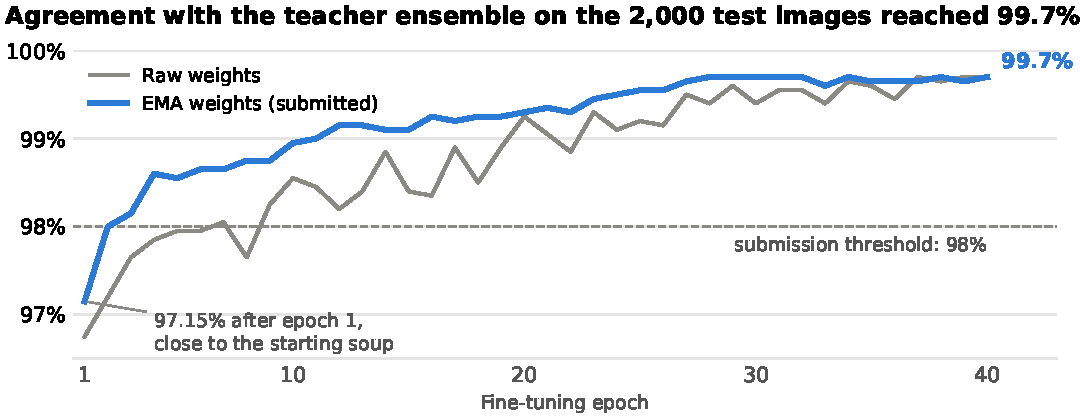
\includegraphics[width=0.88\linewidth]{fig2_agreement.pdf}
\caption{Agreement between the student and the five-model teacher ensemble on the 2,000 test images during round 6, for the EMA (submitted) and raw weights.}
\label{fig:agree}
\end{figure}

The method is cheap and still ships one network under the 5M limit. Its ceiling is the ensemble: once agreement is near 100\%, only better teachers can raise the score.

\section{Results and the final two submissions}
Our best model, the round-6 compressed student, scored \textbf{90.6\% on the public half and 87.5\% on the private half} (about 89.05\% over all 2,000 test images), with \textbf{4,918,602 trainable parameters} and 0.80 GMACs per image, using EMA weights and flip test-time augmentation. It was the best of all our submissions on both halves. Team Transformers finished 24th on the public leaderboard and 26th on the private one.

\textbf{Choosing the final two.} Kaggle ranks each team by the better of its two selected submissions on the private half. We picked (1) the compressed student, which had the highest public score and the strongest evidence behind it, 99.7\% agreement with our most accurate ensemble; and (2) the soup of the round-3 student (0.905 public), which never saw the test images, as a hedge in case the compression gain did not carry over to the private half.

\textbf{What the private half showed.} Every model scored 3--4 points lower on the private half, so those images are harder (Figure~\ref{fig:lb}). The compressed student stayed first, but the others reordered: the two soups, tied second publicly, fell below the SAM and high-resolution students. Compression changed 53 of the 2,000 predicted labels relative to its parent soup, gaining 1 image on the public half (0.905 $\to$ 0.906) but 10 on the private half (0.865 $\to$ 0.875). The public score alone undersold the method.

\begin{figure}[h]
\centering
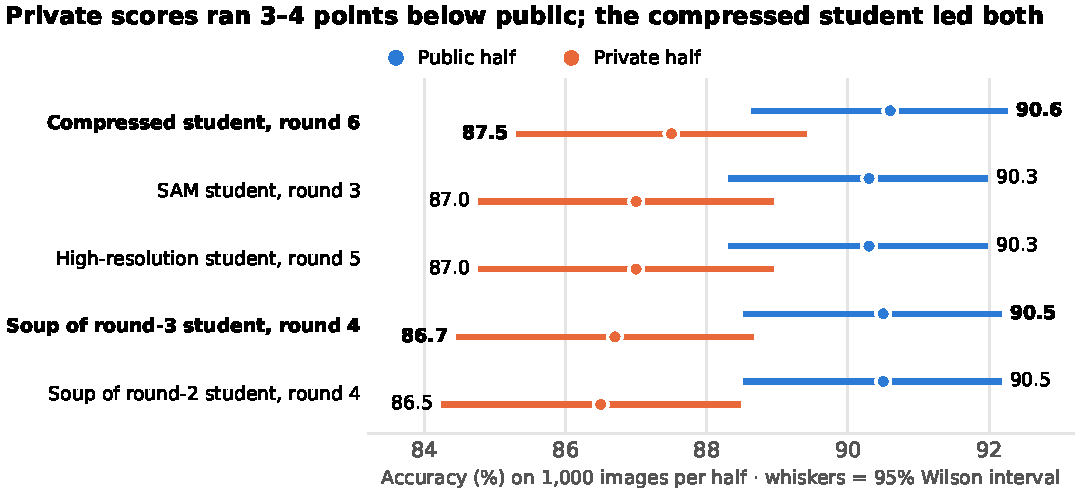
\includegraphics[width=0.88\linewidth]{fig3_public_private.pdf}
\caption{Public and private accuracy of the final pipeline's submissions, with 95\% Wilson intervals for 1,000 images per half. Bold rows are the two final submissions.}
\label{fig:lb}
\end{figure}

\textbf{Where the remaining errors come from.} Relative to an even 200 images per class, the teacher ensemble, the soup and the high-resolution student all predict 17--24 too many automobiles, 20--29 too few airplanes and 12--14 too few frogs. Three different models skewing the same way points to shifted images the training set does not prepare any of them for, not to random mistakes that averaging could cancel (the even split is an assumption, since test labels are hidden).

\section{Lessons learned}
\begin{enumerate}
\item \textbf{Measure the noise before chasing it.} One leaderboard image is worth 0.1 points, and a 95\% interval spans about $\pm$1.9 points. After round 1, every idea changed the public score by less than that, and the private half reordered our models. Choose submissions on method and evidence, not on a 0.001 public difference.
\item \textbf{The teachers set the ceiling.} The same student scored 0.890 with weaker teachers and 0.904 with stronger ones, and once compression reached 99.7\% agreement only better teachers could add more. Reaching 0.92 would have needed an ensemble roughly 1.5 points more accurate on the shifted images, which meant more, and more diverse, teachers than our remaining GPU time allowed.
\item \textbf{A parameter limit is not a compute limit.} Teachers of any size, extra computation per parameter and the unlabelled test images were all usable under the rules. Distillation and compression, which exploit the first and the last, gave our biggest gains.
\item \textbf{Keep an offline yardstick, but know its limits.} A held-out split let us judge SAM cleanly, and we lost it from round 2 by training on all 50,000 images. Yet held-out images resemble the training data: changes worth 0.3--0.5 points there sometimes gave nothing on the shifted test set.
\item \textbf{Infrastructure is part of the method.} A throttling laptop GPU ran about 10$\times$ slower than an A100. Checkpoints every 5--10 epochs rescued a 500-epoch run when the cluster stopped its machine early, and explicit checks on file sizes and exit codes ended two silent pipeline failures.
\end{enumerate}
If we started again, we would fix a held-out split and evaluation protocol on day one, train stronger and more diverse teachers early, and ask the course staff at the start whether unlabelled test-time adaptation is allowed.

\section{Limitations, disclosures and contributions}
\textbf{Use of the unlabelled test images.} The round-6 model was fine-tuned on the 2,000 competition test images, without labels, to match the teacher ensemble's predictions on them. No test labels exist in the competition data and none were used; no pretrained weights or outside data were involved. The model is fitted to this test set, and a new test set would need the 9-minute fine-tune repeated. Our other final submission never saw the test images.

\textbf{Parameter budget.} Both final submissions have 4,918,602 trainable parameters; the teachers (10.4M and 18.5M) only produce training targets, as the project brief allows.

\textbf{Single runs.} Each round was run once with one seed, so differences of a few images carry no variance estimate.

\textbf{Contributions.} Kalp Patel designed the network and ran rounds 0--5 (teachers, distilled students, SAM, model soups and the high-resolution student). Rishi Ajith ran the parallel pipeline and round 6, the ensemble compression.

\section*{References}
\footnotesize
\begin{itemize}[leftmargin=1em,label={}]
\item Beyer, L., Zhai, X., Royer, A., Markeeva, L., Anil, R. \& Kolesnikov, A. (2022). Knowledge distillation: A good teacher is patient and consistent. \emph{CVPR}.
\item Foret, P., Kleiner, A., Mobahi, H. \& Neyshabur, B. (2021). Sharpness-Aware Minimization for efficiently improving generalization. \emph{ICLR}.
\item He, K., Zhang, X., Ren, S. \& Sun, J. (2016). Deep residual learning for image recognition. \emph{CVPR}.
\item Hinton, G., Vinyals, O. \& Dean, J. (2015). Distilling the knowledge in a neural network. \emph{NeurIPS Deep Learning Workshop}.
\item Miller, J., Taori, R., Raghunathan, A., Sagawa, S., Koh, P.\,W., Shankar, V., Liang, P., Carmon, Y. \& Schmidt, L. (2021). Accuracy on the line. \emph{ICML}.
\item M\"uller, S.\,G. \& Hutter, F. (2021). TrivialAugment: Tuning-free yet state-of-the-art data augmentation. \emph{ICCV}.
\item Recht, B., Roelofs, R., Schmidt, L. \& Shankar, V. (2018). Do CIFAR-10 classifiers generalize to CIFAR-10? \emph{arXiv:1806.00451}.
\item Szegedy, C., Vanhoucke, V., Ioffe, S., Shlens, J. \& Wojna, Z. (2016). Rethinking the Inception architecture for computer vision. \emph{CVPR}.
\item Wortsman, M. et al.\ (2022). Model soups: averaging weights of multiple fine-tuned models improves accuracy without increasing inference time. \emph{ICML}.
\item Yun, S., Han, D., Oh, S.\,J., Chun, S., Choe, J. \& Yoo, Y. (2019). CutMix: Regularization strategy to train strong classifiers with localizable features. \emph{ICCV}.
\item Zhong, Z., Zheng, L., Kang, G., Li, S. \& Yang, Y. (2020). Random erasing data augmentation. \emph{AAAI}.
\end{itemize}

\end{document}
